
The first system to be investigated was the Stabilizer circuits constructed by Blake and Linden \cite{Blake2020}. The system is encoded in an $N \times 2N$ matrix or stabilizer tableau, initialised for the all-$X$ string, $X_1, X_2, \dots, X_N$. A random unitary circuit, constructed from the gates, $\mathbf{Z.H}$ and $\mathbf{C3}$, for a circuit depth of $t=20000$. The entanglement entropy is calculated at each time step via (refeq) and plotted against time to produce FIG. \ref{Bal}. The maximum entanglement entropy is found to saturate at the Page value \cite{Page_1993}, signalling a maximally entangled system. Note that the inclusion of $\mathbf{SWAP}$ does not affect any entanglement dynamics, and is omitted from the circuit. We also find that any intially local string of operators, e.g $I\dots X \dots I$ does not generate any entanglement within the system.

\begin{figure}[t!]
    \centering
    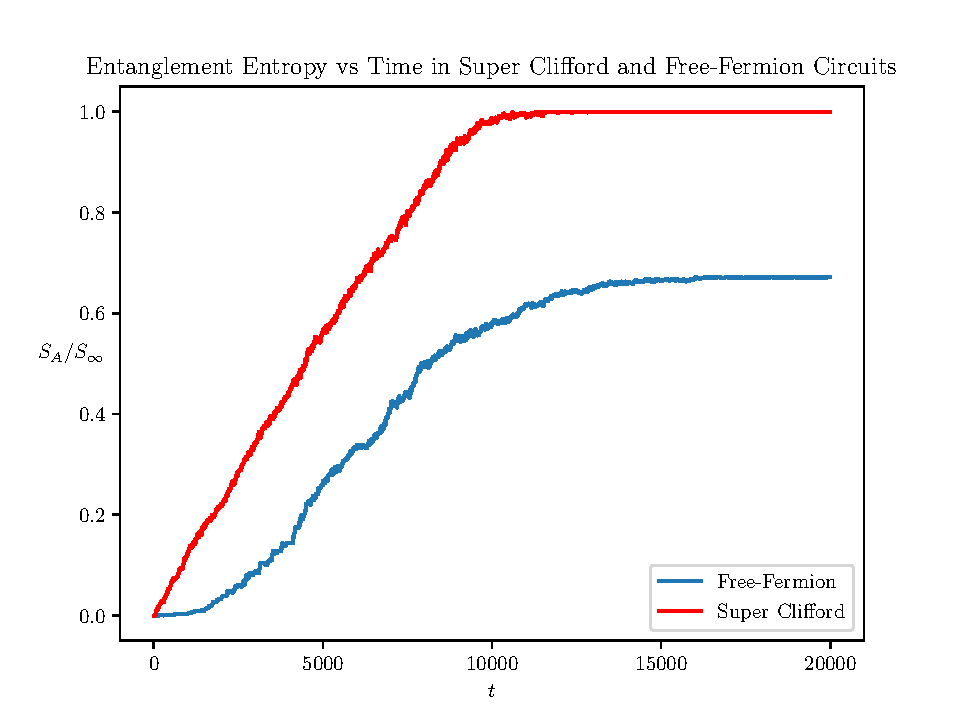
\includegraphics[width=0.48\textwidth]{reportimages/CliffvsFerm.pdf}
    \caption{Comparison of the operator entanglement entropy as a fraction of the maximum entanglement entropy $S_{\infty}$ for a $N = 120$ qubit super-Clifford circuit and a $L = 120$ site, non-interacting fermion circuit. Clifford circuit is constructed from the $\mathbf{Z.H}$ and $\mathbf{C3}$ gates. The non-interacting fermion circuit is constructed from the $G(i, j)$ gate to act on an initially half filled state corresponding to $M^{\text{block}}$. }
    \label{Bal}
\end{figure}
\begin{figure}[h!]
    \centering
    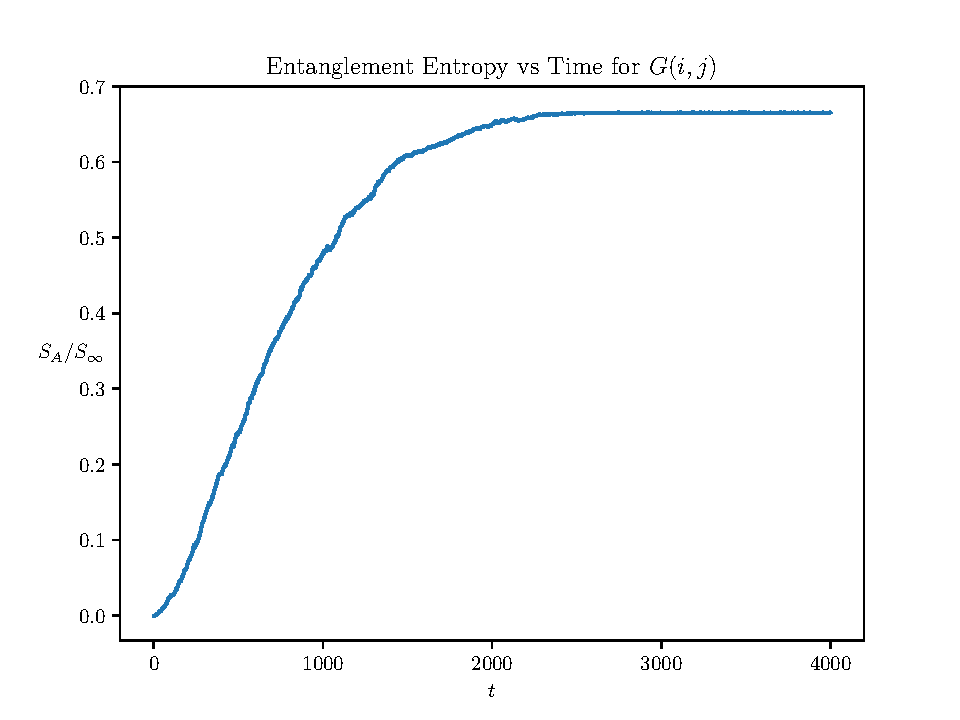
\includegraphics[width=0.48\textwidth]{reportimages/GFock120.pdf}
    \caption{Operator entanglement entropy as a fraction of the maximum entanglement entropy of a fermionicsystem with $L = 120$ modes subject to a non-interacting fermionic circuit of $G(i, j)$. Initial configuration of the system is the alternately-filled state corresponding to $M^{\text{half}}$.}
    \label{halffig}
\end{figure}



\begin{figure}[h!]
    \centering
    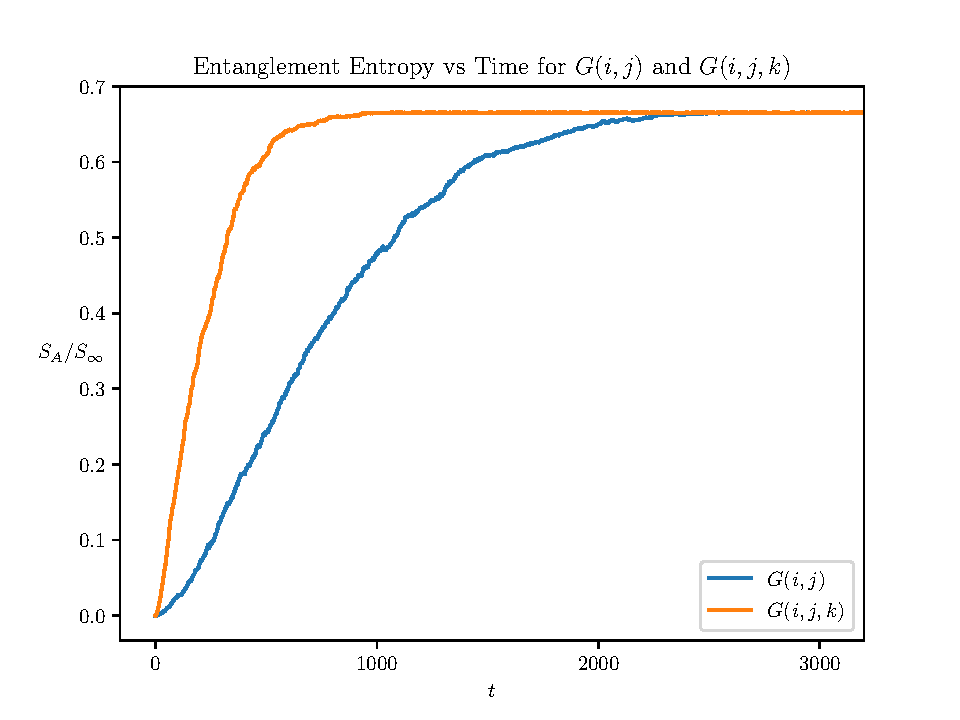
\includegraphics[width=0.48\textwidth]{reportimages/GZFockState120.pdf}
    \caption{Comparison of the operator entanglement entropy as a fraction of the maximum entanglement entropy of fermionic systems with $L = 120$ modes subject to non-interacting fermionic circuits of $G(i, j)$ and $G(i, j, k)$. Initial configuration of the system is the alternately-filled state corresponding to $M^{\text{half}}$.}

    \label{comp}
\end{figure}

\begin{figure}[h!]
    \centering
    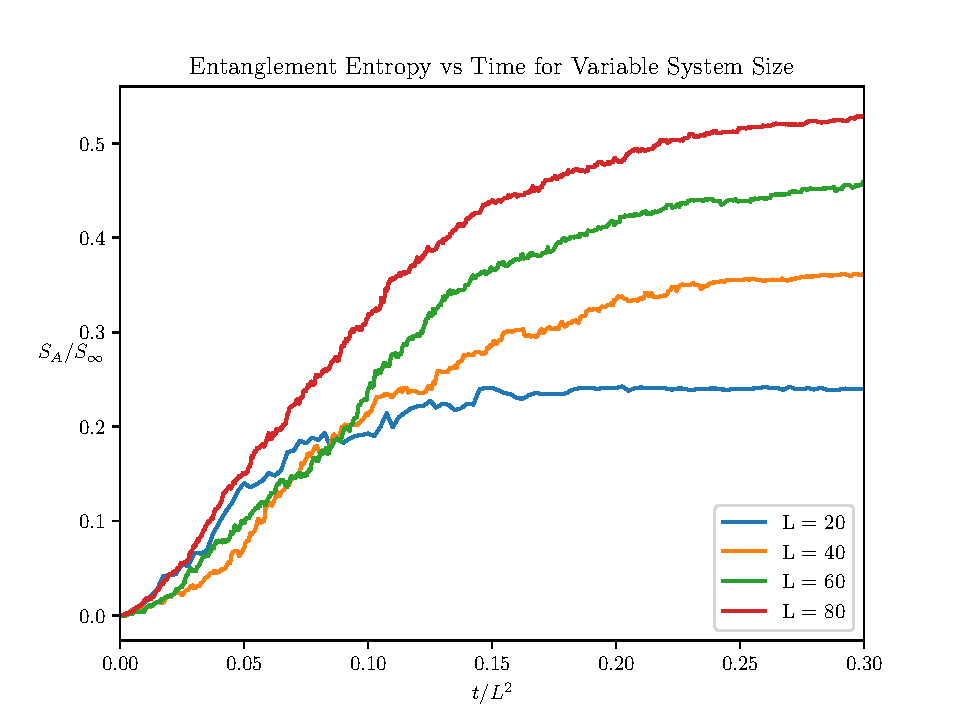
\includegraphics[width=0.48\textwidth]{reportimages/varysystem.pdf}
    \caption{Comparison of the operator entanglement entropy for fermionic systems of varying sizes, ($L = 20, 40, 60, 80$). $L$ modes are subject to a random non-interacting fermionic circuits of $G(i, j)$ and $G(i, j, k)$. Initial configuration of the system is the alternately-filled state corresponding to $M^{\text{half}}$.}

    \label{vary}
\end{figure}



To compare with super Clifford circuits, systems of $L = 120$ modes were simulated for two configurations under two random unitary circuits, built from $G(i, j)$ and $G(i, j, k)$. 
Each gate was constructed in a simulation of the full state-level description, in order to verify the correct actions and expressions before using techniques to efficiently simulate the fermionic systems. 
 Each circuit was first confirmed to not create entanglement on the vacuum state, corresponding to $M^{\text{vac}}$, and then subsequently simulated on the different filled configurations $M^{\text{half}}$ and $M^{\text{block}}$. The results from the random unitary circuit built from $G(i, j)$ can be seen in Fig. \ref{halffig} and \ref{blockstate}. We find that for both system, the entanglement entropy does not saturate at the maximum Page value. The alternating half-filled state when subject to a random unitary circuit, saturates at $t\sim 2300$, which is considerably lower than the state corresponding to $M^{\text{block}}$, which saturates at $t \sim 16000$. This difference in saturation times, is concisely presented in Fig. \ref{comp}, where saturation level is identical in both circuits, but the circuit built from $G(i, j)$ saturates significantly earlier. Simulations of varying system size were also carried out, and it can be seen that the entanglement saturation is directly dependent on the size of the system. 
\begin{figure}[t!]
    
    \centering
    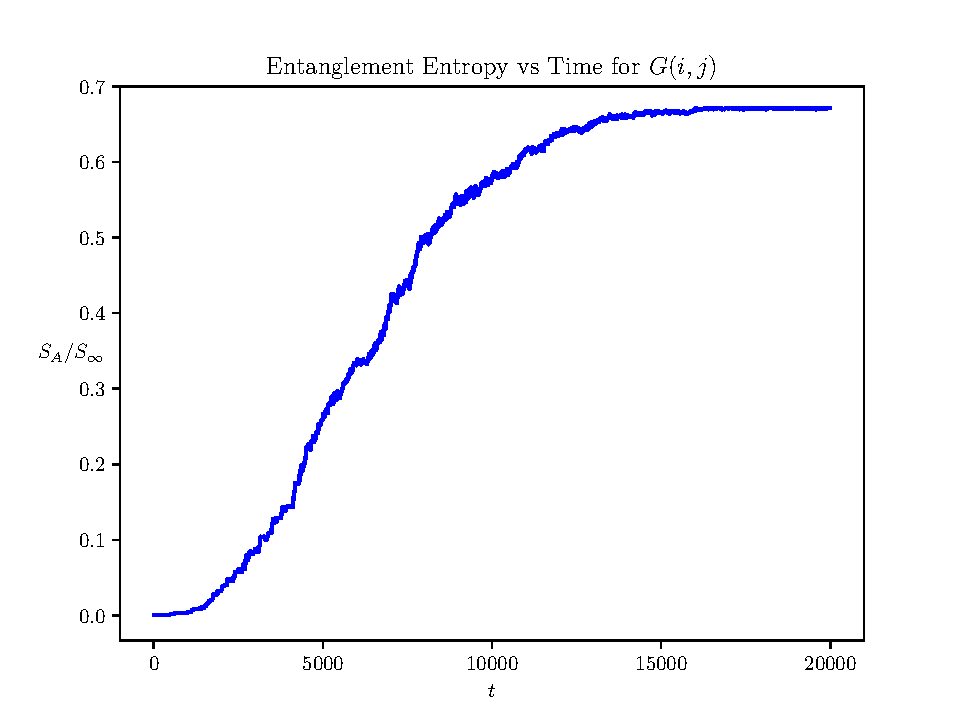
\includegraphics[width=0.48\textwidth]{reportimages/GFerm120.pdf}
    \caption{Operator entanglement entropy as a fraction of the maximum entanglement entropy of a fermionicsystem with $L = 120$ modes subject to a non-interacting fermionic circuit of $G(i, j)$. Initial configuration of the system is the half-filled state corresponding to $M^{\text{Block}}$. }
    \label{blockstate}
\end{figure}







